\documentclass{article}
\usepackage{graphicx}
\usepackage{fullpage}
\usepackage{hyperref}
\usepackage{amsmath}
\usepackage{amssymb}
%\usepackage{draftwatermark}

%\SetWatermarkText{DRAFT}
%\SetWatermarkScale{3}
%\SetWatermarkLightness{0.5}

\begin{document}

\title{EP 501 Midterm exam:  Chapters 1,3-5}

\maketitle

~\\
\textbf{Instructions:}  
\begin{itemize}
  \item  Answer all questions
  \item  You may use the course textbook during this exam
  \item  You may log into your computer and use Matlab.
  \item  You may use \emph{your own} course notes for this exam
  \item  You may use my course notes.  
  \item  You may access the course Canvas site during this exam:  \url{https://erau.instructure.com/courses/101937}
  \item  You may visit the course repository:  \url{https://github.com/mattzett/EP501}  
  \item  You \emph{may not} use an internet browser to access search capabilities and internet references.  
\end{itemize}


\pagebreak

\begin{enumerate}
  \item Use the Taylor Series method (\S 5.4 in the textbook) to develop derivatives for a \emph{nonuniform} (unequally spaced) grid consisting of the three points $x_{i-1},x_i,x_{i+1}$ and function values at those points $f_{i-1},f_i,f_{i+1}$ defined by:
    \begin{eqnarray}
      x_{i-1} &=& x_i - \Delta x_b \\
      x_{i+1} &=& x_i + \Delta x_f \\
      \left( \Delta x_b \right. &\ne& \left. \Delta x_f \right) \\
      f_{i-1} &=& f(x_i - \Delta x_b) \\ 
      f_{i+1} &=& f(x_i + \Delta x_f)     
    \end{eqnarray}
    
    \bigbreak
    
    \begin{itemize}
      \item[(a)]  Develop a \emph{centered} difference approximation for the first derivative with respect to $x$ at the $i^{th}$ grid point, i.e. derive an approximation for:
      \begin{eqnarray}
      f'(x_i) = \left[ \frac{d f}{d x} \right]_i
      \end{eqnarray}
  
    $$f(x + \Delta x_f) = f(x_i) + \Delta x_f f^{'}(x_i) + \frac{\Delta x^{2}_f}{2} f^{''} (x_i) + ... $$
    
    $$f(x - \Delta x_b) = f(x_i) - \Delta x_b f^{'}(x_i) + \frac{\Delta x^{2}_b}{2} f^{''} (x_i) + ... $$
    
    $$f(x + \Delta x_f) - f(x - \Delta x_b) = (\Delta x_f + \Delta x_b)f^{'}(x_i) + \frac{1}{2} (\Delta x^{2}_f - \Delta x^{2}_b)f^{''}(x_i) + ...$$
    
    $$\boxed{f^{'} = \frac{f(x + \Delta x_f) - f(x - \Delta x_b)}{\Delta x_f + \Delta x_b} = \frac{f_{i+1} - f_{i-1}}{\Delta x_f + \Delta x_b}}$$
    
    \bigskip
    \bigskip
    
    \item[(b)]  Show that the truncation error for your finite difference formula is $\mathcal{O}(\Delta x_f - \Delta x_b)$
    Truncated Part of $f^{'}$ :
    $$\frac{\frac{1}{2} (\Delta x^{2}_f - \Delta x^{2}_b)f^{''} (x_i)}{\Delta x_f + \Delta x_b} = \frac{\frac{1}{2} ((\Delta x_f + \Delta x_b)(\Delta x_f - \Delta x_b))f^{''} (x_i)}{\Delta x_f + \Delta x_b}$$
    
    $$ = \frac{1}{2} (\Delta x_f - \Delta x_b)f^{''} (x_i)$$
    Therefore, truncation error is $\boxed{\mathcal{O}(\Delta x_f - \Delta x_b)}$
    
    \pagebreak
    
    \item[(c)]  Obtain an approximate second derivative:
      \begin{eqnarray}
        f''(x_i) = \left[ \frac{d^2 f}{d x^2} \right]_i
      \end{eqnarray}        
      by iteratively applying your first derivative formula derived from part (a), e.g.:
      \begin{eqnarray}
        \left[ \frac{d^2 f}{d x^2} \right]_i \approx 
        \frac{
        \left[ \frac{d f}{d x} \right]_{i+1/2} - \left[ \frac{d f}{d x} \right]_{i-1/2}
        }{x_{i+1/2}-x_{i-1/2}}
      \end{eqnarray} 
    \end{itemize}
    
    $$x_{i+\frac{1}{2}} = x_i + \frac{1}{2} \Delta x_f$$  $$x_{i-\frac{1}{2}} = x_i - \frac{1}{2} \Delta x_b$$
    $$x_{i+\frac{1}{2}} - x_{i-\frac{1}{2}} = \frac{1}{2} (\Delta x_f + \Delta x_b)$$
    
    \bigskip
    
    $$\left[ \frac{d f}{d x} \right]_{i+1/2} = \frac{\displaystyle f_{i + \frac{3}{2}} - f_{i - \frac{1}{2}}}{\displaystyle \Delta x_f + \Delta x_b}$$
    
    $$\left[ \frac{d f}{d x} \right]_{i-1/2} = \frac{\displaystyle f_{i + \frac{1}{2}} - f_{i - \frac{3}{2}}}{\displaystyle \Delta x_f + \Delta x_b}$$
    
    $$\left[ \frac{d^{2} f}{d x^{2}} \right]_{i} = \frac{
    \frac{\displaystyle f_{i + \frac{3}{2}} - f_{i - \frac{1}{2}}}{\displaystyle \Delta x_f + \Delta x_b} - \frac{\displaystyle f_{i + \frac{1}{2}} - f_{i - \frac{3}{2}}}{\displaystyle \Delta x_f + \Delta x_b}}
	{\Delta x_f + \Delta x_b}$$
	
	$$\boxed{\left[ \frac{d^{2} f}{d x^{2}} \right]_{i} = \frac{2\left[ f_{i + \frac{3}{2}} + f_{i - \frac{3}{2}} - f_{i + \frac{1}{2}} - f_{i - \frac{1}{2}} \right]}{(\Delta x_f + \Delta x_b)^{2}}}$$
    
    \pagebreak
    
    \item  Derive and explain matrix condition numbers.  
    \begin{itemize}
      \item[(a)]Use a method similar to that presented in \S 1.6.3.2 to show that the condition number relates variations in the solution vector $\underline{b}$ to variations in the matrix $\underline{\underline{A}}$ via the formula:
      \begin{equation}
      \frac{\left\| \delta \underline{b} \right\|}{ \left\| \underline{b} \right\| } \le   \mathcal{C} (\underline{\underline{A}}) \frac{ \left\| \delta \underline{\underline{A}}   \right\| }{\left\| \underline{\underline{A}} \right\|}
      \end{equation}
      where $\mathcal{C} (\underline{\underline{A}})$ is the condition number of the matrix $\underline{\underline{A}}$.
      
      \medskip
      
      $$\underline{\underline{A}} \underline{x} = \underline{b}$$
      $$(\underline{\underline{A}} + \underline{\underline{\delta A}}) \underline{x} = (\underline{b} + \underline{\delta b})$$
      Subtract first equation from second equation:
      $$\underline{\underline{\delta A}} \underline{x} = \underline{\delta b}$$
      Multiply both sides by $\underline{\underline{A}}^{-1}$:
      $$\underline{\underline{A}}^{-1} \underline{x} = \underline{\underline{A}}^{-1} \underline{\delta b}$$
      $$\underline{\delta b} = \underline{\underline{A}} \underline{\underline{A}}^{-1} \underline{\delta x}$$
      $$C(A) = \underline{\underline{A}} \underline{\underline{A}}^{-1}$$
      Apply Schwarz inequality and divide both sides by $\left\| \underline{\delta b} \right\|$:
      $$\frac{\left\| \delta \underline{b} \right\|}{ \left\| \underline{b} \right\| } \le   \mathcal{C} (\underline{\underline{A}}) \frac{ \left\| \underline{\underline{\delta A}}   \right\| \left| \underline{x} \right|}{\left\| \underline{b} \right\|}$$
      Multiply right side by $\frac{\left|\left| \underline{\underline{A}} \right|\right|}{\left|\left| \underline{\underline{A}} \right|\right|}$:
      $$\frac{\left\| \delta \underline{b} \right\|}{ \left\| \underline{b} \right\| } \le   \mathcal{C} (\underline{\underline{A}}) \frac{ \left\| \underline{\underline{\delta A}}   \right\| \left| \underline{x} \right|}{\left\| \underline{b} \right\|} \frac{\left|\left| \underline{\underline{A}} \right|\right|}{\left|\left| \underline{\underline{A}} \right|\right|}$$
      Assume $\left\| \underline{\underline{A}}   \right\| \left| \underline{x} \right| = \left\| \underline{b} \right\|$
      $$\boxed{ \frac{\left\| \delta \underline{b} \right\|}{ \left\| \underline{b} \right\| } \le   \mathcal{C} (\underline{\underline{A}}) \frac{ \left\| \delta \underline{\underline{A}}   \right\| }{\left\| \underline{\underline{A}} \right\|}}$$
      
            
    \item[(b)] Provide a brief (several sentence) explanation of the meaning of the condition number $\mathcal{C}(\underline{\underline{A}})$.  Include a discussion of what large and small condition numbers mean and why they are undesirable.  
    
    \medskip
    
     \quad The condition number of $\underline{\underline{A}}$ is a measure of the sensitivity to small changes in the system. If the number is large, then small changes in $\underline{\underline{A}}$ will result in large changes to $\underline{b}$. If the number is small, the system is resistant to small changes in $\underline{\underline{A}}$.
    \end{itemize}
    
    \pagebreak
    
    \item \emph{Trilinear} interpolation involves approximation of an underlying three dimensional function using a polynomial of the form:  
    \begin{equation}
      f(x,y,z) \approx a_1 + a_2 x + a_3 y + a_4 z + a_5 x y + a_6 y z + a_7 x z + a_8 x y z
    \end{equation}
    for the region $x_i \le x \le x_{i+1}, y_j \le x \le y_{j+1}, z_k \le x \le z_{k+1}$.  Set up a system of equations that can be solved for the coefficients $\underline{a} \equiv a_\ell$ using the value of the function $f$ at the eight points defining the vertices of this cube-shaped region, shown in the diagram below.  Express your system of equations in matrix form.  \\~\\~\\
    %\begin{figure}{h*}
    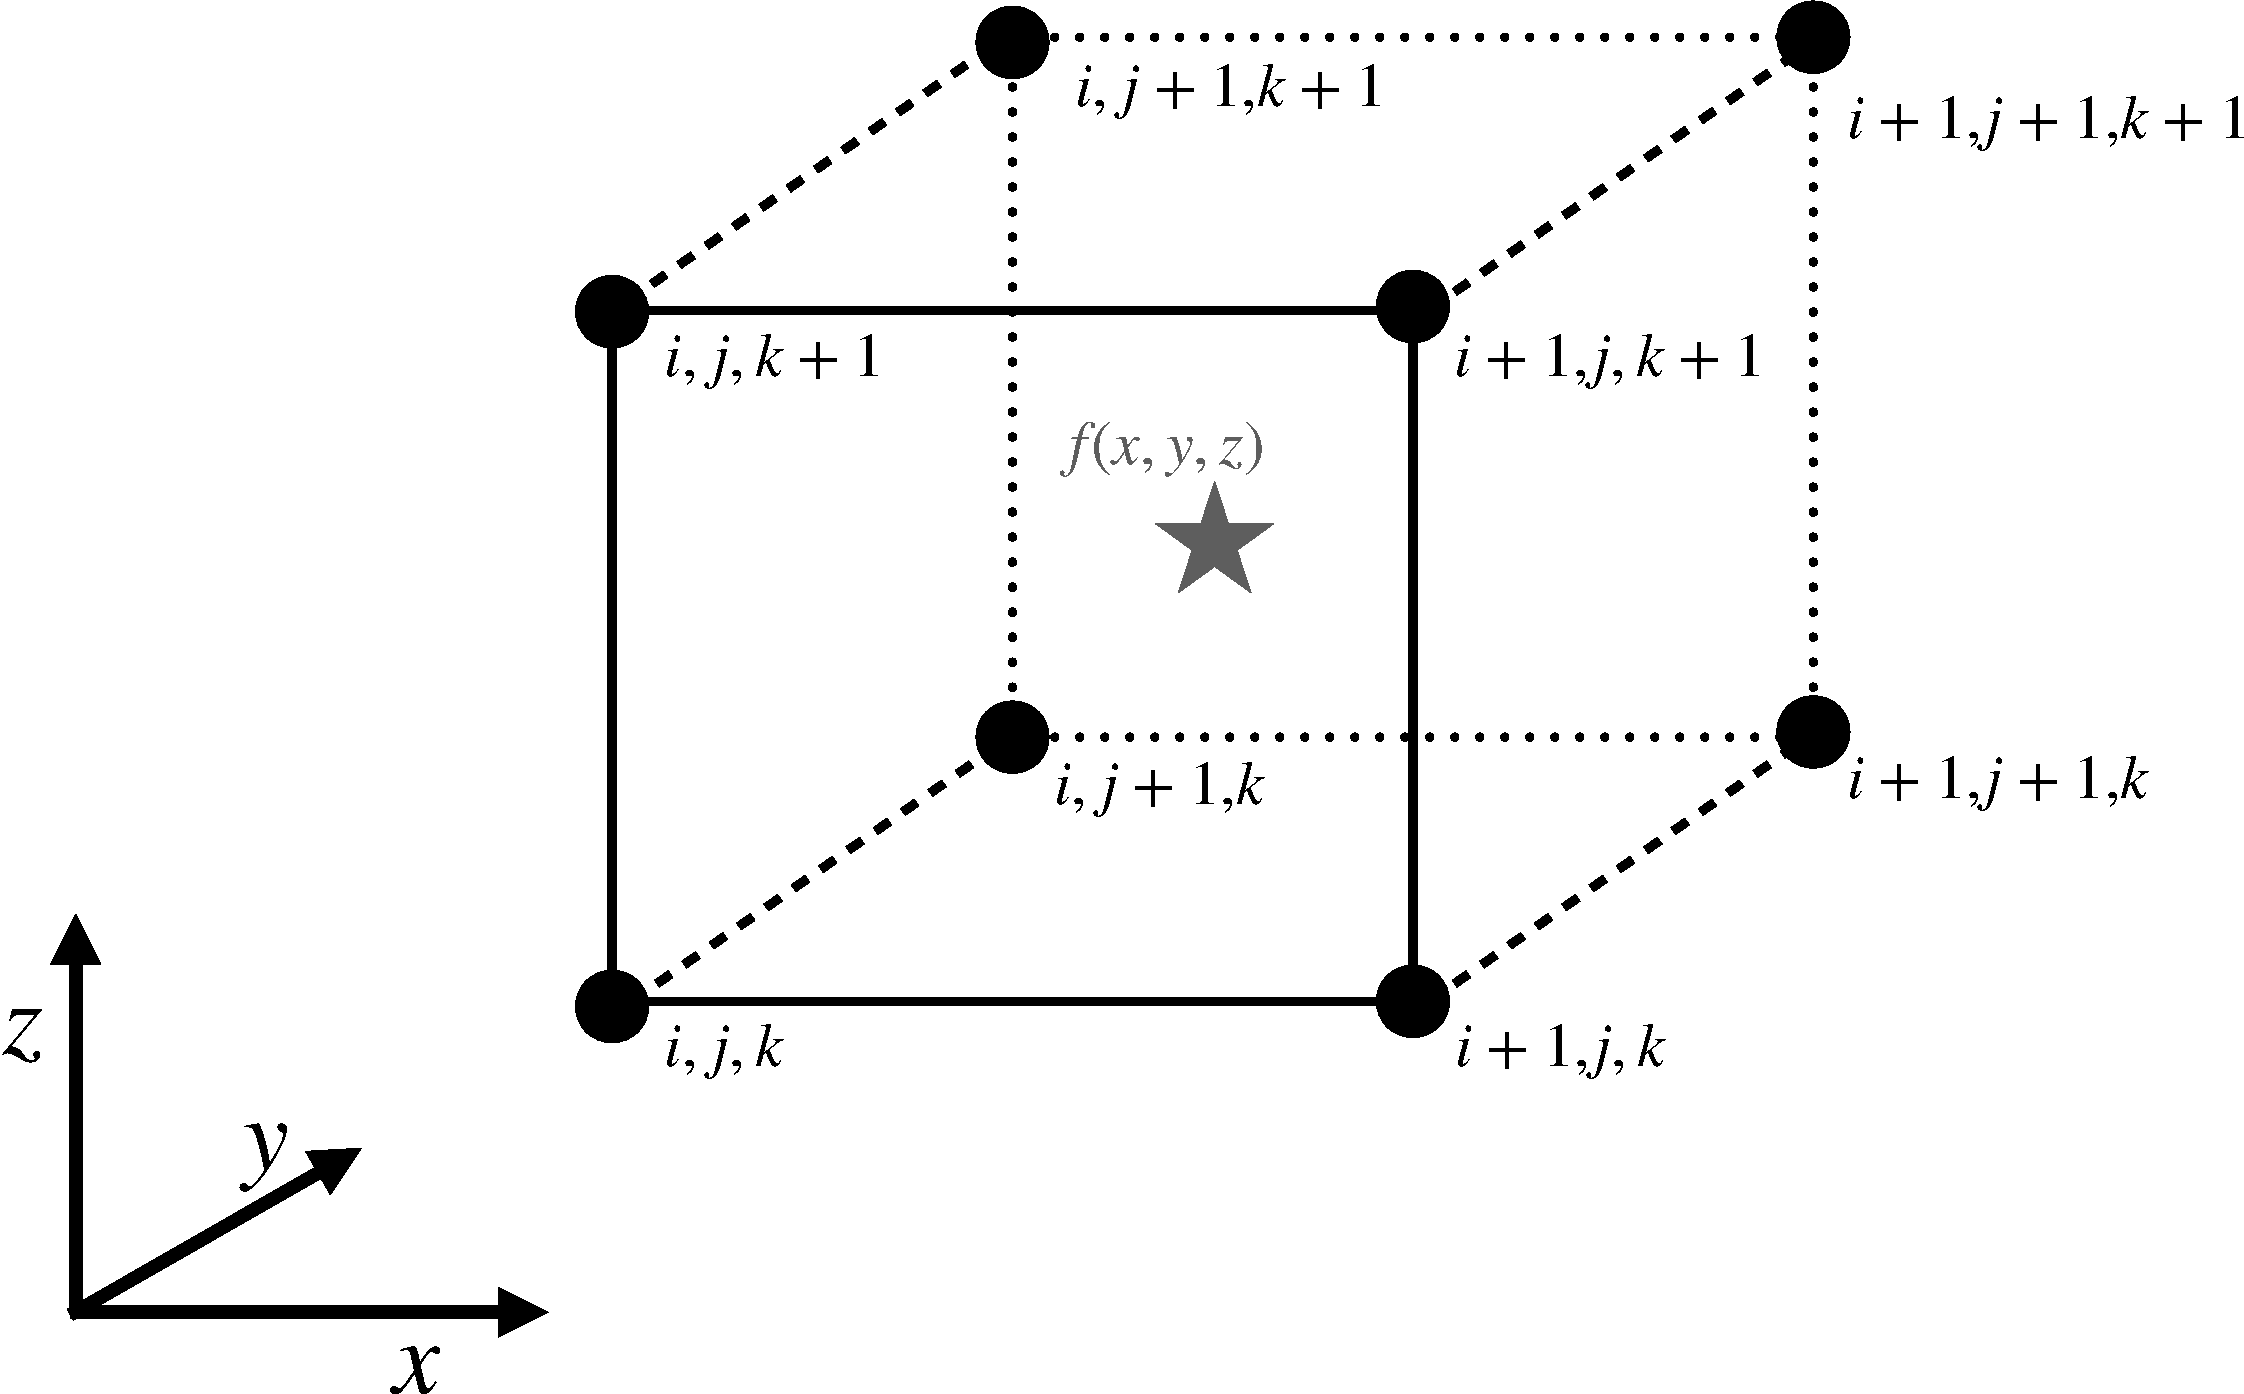
\includegraphics[width=0.5\textwidth]{diagram_trilinear-crop.pdf}
    %\end{figure}
    
    $$\underline{\underline{M}} = 
     \begin{bmatrix}
    	1 & x_1 & y_1 & x_1 y_1 & y_1 z_1 & x_1 z_1 & x_1 y_1 z_1 \\	
    	1 & x_2 & y_2 & x_2 y_2 & y_2 z_2 & x_2 z_2 & x_2 y_2 z_2 \\
    	1 & x_3 & y_3 & x_3 y_3 & y_3 z_3 & x_3 z_3 & x_3 y_3 z_3 \\
    	1 & x_4 & y_4 & x_4 y_4 & y_4 z_4 & x_4 z_4 & x_4 y_4 z_4 \\
    	1 & x_5 & y_5 & x_5 y_5 & y_5 z_5 & x_5 z_5 & x_5 y_5 z_5 \\
    	1 & x_6 & y_6 & x_6 y_6 & y_6 z_6 & x_6 z_6 & x_6 y_6 z_6 \\
    	1 & x_7 & y_7 & x_7 y_7 & y_7 z_7 & x_7 z_7 & x_7 y_7 z_7 \\
    	1 & x_8 & y_8 & x_8 y_8 & y_8 z_8 & x_8 z_8 & x_8 y_8 z_8 \\
    \end{bmatrix}$$
    
    $$\underline{a} = \begin{bmatrix}
    a_1 \\
    a_2 \\
    a_3 \\
    a_4 \\
    a_5 \\
    a_6 \\
    a_7 \\
    a_8 \\
    \end{bmatrix} , \underline{f} = \begin{bmatrix}
    f_1 \\
    f_2 \\
    f_3 \\
    f_4 \\
    f_5 \\
    f_6 \\
    f_7 \\
    f_8 \\
    \end{bmatrix}$$
    
    $$\underline{\underline{M}} \underline{a} = \underline{f}$$
    
    \pagebreak
    
   \item Suppose we wish to perform a least squares fit (\S 4.10) to a set of measurements $y_i$ sampled at independent variable locations $x_i$ using the functional form:  
    \begin{equation}
      y(x) = a x^2 + b x^5
    \end{equation}
    Derive a system of equations can can be solved to determine the coefficients $a,b$.  Express your system in matrix form.  
     
    \bigskip
    
    \bigskip
    
    No corrections needed, see attached exam.
    
\end{enumerate}

\end{document}